\begin{appendices}
\chapter{Chapter \ref{chp:4} supplementary material} \label{app:chap4}

This section discusses if the chosen estimators presented in Chapter \ref{chp:4:1} have satisfying proprieties in presence of left censored data. We will first present the hypothesis we mace on the change-point model and use some elements of the demonstration made in \cite{Lavielle1997} to proove that the estimators $\widehat{K}$ and $\widehat{\TT}$ still converge in the censored setting. Then, we study the convergence of a segment parameters and the importance of the initialization value in the Newton-Raphson method. In the third section, we will check if the necessary conditions to use the PELT algorithm are verified. The last part will be dedicated to the experiments on the estimation procedure proposed in \ref{chp:4:3}. 

\section{Elements of proof of convergence of the parametric change-point detection model}\label{app:chap4:1}

The hypothesis on the change-point model are the following:  
\begin{itemize}
\item[\textbf{H1:}] $\Theta$ is compact and there exists $\Delta_{\bm \theta}^{\star}>0$ such that $\vert \theta_{k+1}^{\star}-\theta_{k}^{\star}\vert > \Delta_{\bm \theta}^{\star}$, for all $k=0,...,K^{\star}$.
\item[\textbf{H2:}] There exists $\Delta_{\bm \tau}^*>0$ such that $\vert \tau_{k}^{\star}-\tau_{k-1}^{\star}\vert > \Delta^*_{\bm \tau}$, for all $k=1,...,K^{\star}$.
\item[\textbf{H3:}]  The maximum number of regimes may be written as $K_{\max} \geq \frac{n}{\Delta^*_{\bm \tau}}$. 
\item[\textbf{H4:}] The penalty value is dependant of $n$. It can be written $\beta_{n}$ and verifies $\beta_{n}\xrightarrow[n\rightarrow \infty]{} \infty$ and $\frac{\beta_{n}}{n}\xrightarrow[n\rightarrow \infty]{} 0$.
\end{itemize}

These are classical hypothesis that one can find in \cite{Lavielle1997} or \cite{He2010}. Hypothesis \textbf{H1} mainly aims at ensuring sufficient conditions for the identifiability of the model, by imposing a minimum gap between two consecutive $\theta$'s. We have seen in Section \ref{chp:4:2} that censorship could cause some problem with the identifiability. However, the introduction of a maximum value for parameter $\theta$ solved this problem. Hypothesis \textbf{H2} checks that each regime contains sufficient data for obtaining reliable estimates for the $\theta$'s and Hypothesis \textbf{H3} states the number of regimes is bounded from above. Hypothesis \textbf{H4} is verified by a large range of penalties. The penalty value is not set in our procedure since we explore a range of values $[\beta_{min},\beta_{max}]$ with the CROPS algorithm. However, this range of values is chosen using the BIC criterion \citep{YAO1988181} which verifies assumption \textbf{H4}. In change point detection, the BIC penalty can be written as: 
$$\beta_{BIC} = \frac{D\log(n)}{2},$$
with $D$ the dimension of the parameters $\theta$ and $n$ the length of signal $\bm y$. The penalty range value explored in this thesis writes under the form: 
$$[\beta_{min},\beta_{max}] = [\frac{\beta_{BIC}}{j},\beta_{BIC}\times j],$$
with $j\in\mathbb{N}$. Hence, our penalty range is calibrated accordingly to Hypothesis \textbf{H4} because $\beta_{min}$ and $\beta_{max}$ also verifies its conditions.  

An additionnal hypothesis, which is also the strongest one, implies that change-point locations are independent of the scale and frequency at which the data is sampled. This hypothesis will also allow us to derive the asymptotic behaviour of the estimate, when the sample size is sufficiently large. One should note here that a larger sample means a finer scale for sampling the data and not an extension of the period of observation. The scale of sampling being one of the main problem of the data we are working with, it is hard to verify. However, we can suppose that the change-points occuring in concentration data are linked with the farming activities and the phyto-pharmaceutical uses. Those events happen in fixed moments in times, thus invariant with the sampling rate. 


The proof of convergence of \ref{chp:4:estim} is based our demonstration entirely on the approach developped in \cite{Lavielle1997}. The most critical element in the proof is the condition C0(h) of \cite{Lavielle1997}. We introduce another condition. But first let's denote $\eta_i = \ln f(Y_i,\theta_{k})-\mathbbm{E}[\ln f(Y_i,\theta_{k})]$ for $i$ belonging to the $k$-th segment and associated to the parameters $\theta_{k}$. We have the following proposition: 
 
\begin{proposition}
     There exists $C < \infty$ such that for any $t\geq 0$ and any $s > 0$,
     \begin{equation}\label{app:C0}
     \mathbbm{E}[\sum_{i=t+1}^{t+s}\eta_i]^2\leq Cs^h,    
     \end{equation}
     for some $1\leq h\leq 2$.
\end{proposition}

In \citep{Lavielle1997}, an indication is given that this condition is indeed verified in our case. It explains that in the application framework, if the base signal of $(Y_1,...,Y_n)$ is generated by independent variables, then the variable $\eta_i$ is also a sequence of random variables and the proposition is verified for $h = 1$. Then from Theorem 2.2 of \cite{Lavielle1997}, we have the consistency of the estimator: 
$$ (\widehat{\TT}, \widehat{\bm \theta}) \xrightarrow[n\rightarrow \infty]{\PP^{\star}}   (\bm\TT^{\star}, \bm \theta^{\star})$$
Although $(Y_1,...,Y_n)$ is not i.i.d., the censoring threshold makes the support of this random variables differ, the base signal is emanating from $(C_1,...,C_n)$ that is defined in \ref{chp:4:1} and that is i.i.d..  

\section{Newton-Raphson initialization experiments}\label{app:chap4:2}

We show in this section that the initialization value is an important parameter when estimating the segment parameters with numerical methods such as Newton-Raphson. We illustrate this fact with the Weibull distribution.
We propose to test out four initialisation values in the Newton-Raphson algorithm. We can choose between the classical techniques such as the moment method estimator $\lambda_{init}^{MM}$ \cite{Johnson1994}, the quantile inversion estimator $\lambda_{init}^{QI}$, the weighed maximum likelihood estimator $\lambda_{init}^{WMLE}$ \cite{sadani2019new} or the classical maximum likelihood estimator $\lambda_{init}^{MLE}$ of a Weibull scale parameter. Supposing a sample of observations $\bm x = (x_1,...,x_n)$ generated from a left censored Weibull of parameters $(\lambda,\sigma)$ and censoring threshold $a$, we can define them as follow : 
    %\begin{align*}
    \begin{itemize}
        \item[$\circ$] $\lambda_{init}^{MM} =\frac{\Gamma(1+\frac{1}{\sigma})}{\bar{\bm x}}$ 
        \item[$\circ$] $\lambda_{init}^{QI} = \frac{\bigg(-\ln(1-\alpha)\bigg)^{\frac{1}{\sigma}}}{q_{\bm x}^\alpha}$
        \item[$\circ$] $\lambda_{init}^{WMLE} = \bigg(\frac{1}{nq^{0.5}_{\mathcal{W}(n,n)}}\sum_{i = 1}^nx_i^\sigma \bigg)^{-\frac{1}{\sigma}}$
        \item[$\circ$] $\lambda_{init}^{MLE} = \bigg(\frac{1}{n}\sum_{i = 1}^nx_i^\sigma \bigg)^{-\frac{1}{\sigma}}$, 
    \end{itemize}
    %\end{align*}
    where $q^{0.5}_{\mathcal{W}(n,n)}$ is the median of Weibull with parameters $(n,n)$, $q_{\bm x}^\alpha$ is the $\alpha$-th empirical quantile of the sample $\bm x$. \\
     Two important points must be noted. First, all the initialisation values depend on $\sigma$. It is not problematic in our simulation tests because it is supposed known and fixed. However it stresses again the necessity of its estimation in the future (see section \ref{chp:4:3}). Second, those estimators do not take the censorship into account. They are all biased (except if the sample $\bm x$ does not bear any censored values). \\
     We tested all possible configurations with the varying values of $n = (20,100,500)$, $\lambda = (1/100,1,100)$ and $a$ depending on a censoring rate $\alpha = (0.05,0.25,0.5,0.75,0.95)$. $a$ was the threshold such that $\alpha \%$ of the sample was censored. The shape parameter is supposed known and fixed at $\sigma = 0.5$. For each cases, we simulated $N = 1000$ samples of left censored Weibull with scale parameter $\lambda$ and censored rate $\alpha$. We then compute the mean of all estimates for each initialisation values. All the results are stored into Tables \ref{tab:sim:init1} and \ref{tab:sim:init2}. The simulations show that all initialisation values lead to extremely similar results. It is worth mentioning that the quantile is not reliable for low values of $n$. In the rest of this work, the initialisation value will be defined as the weighed maximum likelihood. The table for the case where $n = 500$ is not displayed because all methods gave the same results. However, the most important result of this experiment is that the method converges and that the choice of the initialization point is important. From now on, we choose to initialize the method with the weighed Maximum Likelihood Estimator.  s

\begin{table}[ht] 
\centering
\begin{tabular}{|rr||rrrr|}
 \hline
 $\alpha$ & $\lambda$ & $\overline{\hat\lambda}_{WMLE}$ & $\overline{\hat\lambda}_{MLE}$ & $\overline{\hat\lambda}_{QI}$ & $\overline{\hat\lambda}_{MM}$ \\
  \hline
  \hline
 0.05 & 100.00 & 116.77 & 116.77 & 1963.08 & 116.77 \\ 
   0.05 & 1.00 & 1.16 & 1.16 & 1.47 & 1.16 \\ 
   0.05 & 0.01 & 0.01 & 0.01 & 1790.22 & 0.01 \\ 
   0.25 & 100.00 & 119.24 & 119.24 & 151.37 & 119.24 \\ 
   0.25 & 1.00 & 1.16 & 1.16 & 2362.08 & 1.16 \\ 
   0.25 & 0.01 & 0.01 & 0.01 & 6038.39 & 0.01 \\ 
   0.50 & 100.00 & 118.07 & 118.07 & 3687.48 & 118.07 \\ 
   0.50 & 1.00 & 1.18 & 1.18 & 1.48 & 1.18 \\ 
   0.50 & 0.01 & 0.01 & 0.01 & 0.02 & 0.01 \\ 
   0.75 & 100.00 & 122.44 & 122.44 & 1724.86 & 122.44 \\ 
   0.75 & 1.00 & 1.25 & 1.25 & 2602.37 & 1.25 \\ 
   0.75 & 0.01 & 0.01 & 0.01 & 1189.03 & 0.01 \\ 
   0.95 & 100.00 & 163.51 & 163.51 & 165.04 & 163.51 \\ 
   0.95 & 1.00 & 1.62 & 1.62 & 1.63 & 1.62 \\ 
   0.95 & 0.01 & 0.02 & 0.02 & 0.02 & 0.02 \\ 
   \hline
\end{tabular}
\caption{Choice of initialisitation value: simulation results for $n = 20$.}\label{tab:sim:init1}
\end{table}

\begin{table}[ht]
\centering
\begin{tabular}{|rr||rrrr|}
\hline
 $\alpha$ & $\lambda$ & $\overline{\hat\lambda}_{WMLE}$ & $\overline{\hat\lambda}_{MLE}$ & $\overline{\hat\lambda}_{QI}$ & $\overline{\hat\lambda}_{MM}$ \\ 
  \hline
  \hline
0.05 & 100.00 & 102.65 & 102.65 & 102.98 & 102.65 \\ 
  0.05 & 1.00 & 1.03 & 1.03 & 1.03 & 1.03 \\ 
  0.05 & 0.01 & 0.01 & 0.01 & 0.01 & 0.01 \\ 
  0.25 & 100.00 & 102.97 & 102.97 & 103.52 & 102.97 \\ 
  0.25 & 1.00 & 1.03 & 1.03 & 1.03 & 1.03 \\ 
  0.25 & 0.01 & 0.01 & 0.01 & 0.01 & 0.01 \\ 
  0.50 & 100.00 & 104.23 & 104.23 & 104.40 & 104.23 \\ 
  0.50 & 1.00 & 1.03 & 1.03 & 1.03 & 1.03 \\ 
  0.50 & 0.01 & 0.01 & 0.01 & 0.01 & 0.01 \\ 
  0.75 & 100.00 & 104.41 & 104.41 & 104.49 & 104.41 \\ 
  0.75 & 1.00 & 1.04 & 1.04 & 1.04 & 1.04 \\ 
  0.75 & 0.01 & 0.01 & 0.01 & 0.01 & 0.01 \\ 
  0.95 & 100.00 & 110.90 & 110.90 & 110.90 & 110.90 \\ 
  0.95 & 1.00 & 1.10 & 1.10 & 1.10 & 1.10 \\ 
  0.95 & 0.01 & 0.01 & 0.01 & 0.01 & 0.01 \\ 
   \hline
\end{tabular}
\caption{Choice of initialisitation value: simulation results for $n = 100$.}\label{tab:sim:init2}
\end{table}

\section{Verifying PELT assumptions}\label{app:chap4:3}

Some necessary conditions must be met before using the PELT algorithm. It can be found in Theorem 3.1 of \cite{Killick2012} and can be stated as follow:  
\begin{proposition}
    We assume that  when  introducing a changepoint into a sequence of observations the  cost, $\mathcal{C}$, of the sequence reduces. More formally, we assume there exists a constant $K$ such that for all $t<s<T$,
    \begin{equation}\label{app:pelt}
      W(y_{t:s}) + W(y_{s:T}) + K \leq W(y_{t:T})  
    \end{equation}
    Then if
    \begin{equation}\label{app:pelt2}
      F(t)+W(y_{t:s})+K \geq F(s)  
    \end{equation}
    holds, at a future time $T>s$, $t$ can never be the optimal last change point prior to $T$.
\end{proposition}

\textbf{Proof:} The equation \ref{app:pelt} is always verified with working with additive criterion such as the log likelihood. We can see that in the case of our cost function: 
$$W(y_{t:s},\hat\lambda_{t:s})+W(y_{s:T},\hat\lambda_{s:T})+K\leq W(y_{t:T},\hat\lambda_{t:T})$$
It is a direct consequence of using the maximum likelihood estimator. Suppose now that \ref{app:pelt2} is true. Adding $W(y_{s:T},\hat\lambda_{s:T})$ on both sides of the inequation gives : 
\begin{align*}
  F(t)+W(y_{t:s},\hat\lambda_{t:s})+W(y_{s:T},\hat\lambda_{s:T})+K &\geq F(s)+W(y_{s:T},\hat\lambda_{s:T}) \\
  \implies F(t)+W(y_{t:T},\hat\lambda_{t:T}) &\geq F(s)+W(y_{s:T},\hat\lambda_{s:T}),
\end{align*}
We can conclude that the segmentation with the smallest cost is the one with $s$ as the last change-point. So $t$ cannot be the last change-point prior to $T$.


\section{Convergence of \texorpdfstring{$\hat\sigma$}{s}}\label{app:chap4:4}

The experimental protocol is the following. We simulated $N = 100$ samples of size $n = 320$ of left censored Weibull realisations. 3 change points are present in the samples at position $80$, $160$ and $240$. The associated parameters for each segment are $(1,1/100,1/100,1)$. Four scenarios are proposed where the $\sigma^*$ and the censoring rate $\alpha$ varies. We test all configuration possible for $\sigma^* = (0.4,0.8)$ and $\alpha = (25\%,75\%)$. All the results are presented in Figures \ref{fig:sim:sigma1} and \ref{fig:sim:sigma2}.     

\begin{figure}[ht]
    \centering
    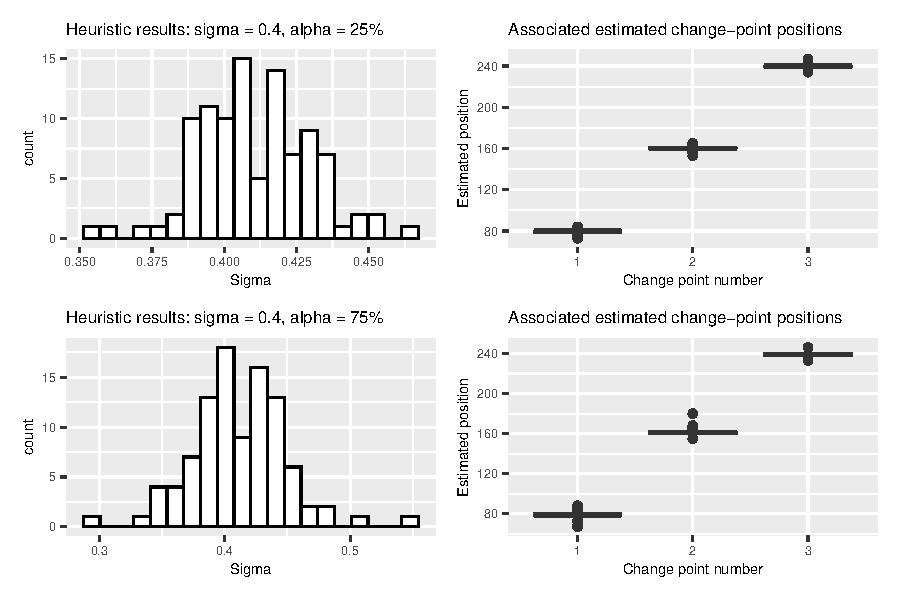
\includegraphics{figs/App/SIM_CHAP5_1.pdf}
    \caption{Scenarios with $\sigma = 0.4$.}
    \label{fig:sim:sigma1}
\end{figure}

\begin{figure}[ht]
    \centering
    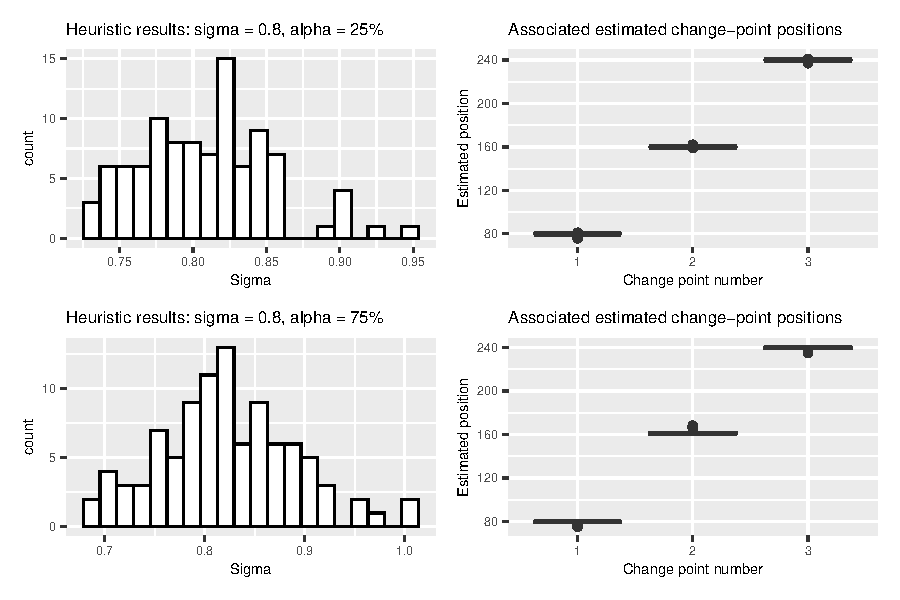
\includegraphics{figs/App/SIM_CHAP5_2.pdf}
    \caption{Scenarios with $\sigma = 0.8$.}
    \label{fig:sim:sigma2}
\end{figure}

For each of these samples, we use the estimation strategy proposed in \ref{chp:4:3}. The penalty grid was defined by $Q = 5$ values set to $[\beta_0 = \frac{\ln n}{10},\dots,\beta_{q},\dots,\beta_{Q} = 5\ln n]$ with the $\beta_q$ being equidistant. We allowed this important range in the penalties to ensure enough distinct points for the elbow heuristic. The minimal segment size was set to 25. The choice was motivated by the computational time of the simulations, even though we have seen that the detection capacity of our method is lower with this minimal segment size. In the procedure, the first iteration $\widehat{\sigma}_0$ is computed with the \texttt{fitdistr} R package \cite{delignette2015}. In the first step of the estimation strategy proposed in \ref{chp:4:3}, minimizing with respect to $\sigma$ is done using \cite{Byrd1995} which allows for a box constraint for the parameter value $\sigma$ (lower and upper bounds). This interval was set to $[0,1]$. This explains that the estimated values are all inferior to 1 in Figure \ref{fig:sim:sigma2}. We defined a stopping criterion to the heuristic depending on the $\widehat{\sigma}$ values that consists in stopping when the upgrade of the new $\widehat{\sigma}$ is not superior to $10^-3$.


\chapter{Chapter \ref{chp:5} supplementary material}\label{app:chap5}

\section{Clustering algorithms}\label{app:clustalgo:chap5}

We keep the same notations than in \ref{section:spaceclust}. We introduce the following new notations : 
\begin{itemize}
    \item $C_m^p$ the $m$-th cluster located in component $p$.
    \item $M_p$ the number of clusters in component $\mathcal{K}_p$.
    \item $\displaystyle Q(\mathcal{K}_p,C_m^p) = \frac{1}{\lvert C_m^p\rvert}\sum_{v_i,v_j \in C_m^p}d_{ij}^2$ the inertia of cluster $C^p_m$.
    \item $\displaystyle R_p(M_p) = \min_{(C_m^p)_{m=1}^{M_p}}\sum_{m = 1}^{M_p}Q(\mathcal{K}_p,C_m^p)$ the best partition (in the sense of minimal inertia) of component $p$ into $M_p$ clusters. 
    \item $\displaystyle S(l,m) = \min_{(M_p)_{p=1}^l \text{ such that } \sum_{p=1}^l M_p = m}\sum_{p=1}^lR_p(M_p)$ which is the best partition of the $l$ first components into a total number of $m$ clusters.
\end{itemize}

$R_p(m)$ can be computed with Ward hierarchical clustering technique. In the case of this work we used the \texttt{R} package \texttt{hclust}. With these notations, we can write the two developed methods as follows: 

\begin{algorithm}[ht]
\caption{Clustering with greedy method:}\label{algo:greed}
\begin{algorithmic}

\State \textbf{input} : the station graph $G=(V,E)$, the known partition into non connex components $(\mathcal{K_1},\dots,\mathcal{K}_P)$, a total number of clusters $M$ \\
  
\State \textbf{initialisation} : Compute $R_p(1)$ for all $p \in [1,\dots,P]$ using \texttt{hclust}, set $M_{opt} = (1,\dots,1)$ vector of size $P$  \\

\For{$m = 1$ to $M-P$}
  \State $\textit{score}\gets(0,\dots,0)$ vector of size $P$
  \For{$p = 1$ to $P$}
  \State $M_{opt}(p) \gets M_{opt}(p) + 1$
  \State $\textit{score}(p) \gets \sum_{p=1}^P R_p(M_{opt}(p))$
  \State $M_{opt}(p) \gets M_{opt}(p) - 1$
  \EndFor
  \State $\textit{pos} \gets which.min(\textit{score})$
  \State $M_{opt}(pos) \gets M_{opt}(pos)+1$
\EndFor
\For{$p=1$ to $P$}
\State built the optimal partition of $\mathcal{K}_p$ with $M_{opt}(p)$ clusters using \texttt{hclust}.
\EndFor

\end{algorithmic}
\end{algorithm} 

\begin{algorithm}[ht]
\caption{Clustering by dynamic programming:}\label{algo:dyn}
\begin{algorithmic}

\State \textbf{input} : the station graph $G=(V,E)$, the known partition into non connex components $(\mathcal{K_1}$, a total number of clusters $M$ \\
    
 \For{$p=1$ to $P$} : 
 \State Use \texttt{hclust} to compute $R_p(m)$ for all $m \in \{1,\dots,M-P+1\}$
 \EndFor 
 \For{$m=1$ to $M-P+1$} : 
 \State $S(1,m) \gets R_1(m)$ 
 \EndFor 
 \For{$l = 2$ to $P$} : 
  \For{$m = l$ to $M$} : 
     \State $W(l,m) \gets 1$ 
     \State $S(l,m) \gets S(l-1,m-1)+R_l(1)$
   \For{$u = 1$ to $m-l+1$}
   \If{$S(l-1,m-u)+R_l(u) < S(l,m)$}
     \State $W(l,m) \gets u$
     \State $S(l,m) \gets S(l-1,m-u)+R_l(u)$
   \EndIf
   \EndFor
 \EndFor 
 \EndFor 
 \State $M_{opt} \gets (\text{NA},\dots,\text{NA})$
 \State $P_{opt}(P) \gets W(P,M)$
 \State $\textit{left} \gets M-W(P,M)$
 \For{$p = P-1$ to $1$}
 \State $P_{opt}(p) \gets W(p,\textit{left})$
 \State $\textit{left} \gets \textit{left}-W(p,\textit{left})$
 \EndFor
 \For{$p = 1$ to $P$}
 \State built the optimal partition of $\mathcal{K}_p$ with $P_{opt}(p)$ clusters using \texttt{hclust}
 \EndFor 
\end{algorithmic}
\end{algorithm} 

\clearpage

\section{Modified empirical Wasserstein distance}\label{appendix:wasserstein}

The Wasserstein distance was chosen over the Kolmogorov-Smirnov or the Jensen-Shannon metric. It has the advantage of integrating in the distance calculation both the differences between the probabilities of observing different values but also the distances between those values. This is a critical point which is illustrated on a simple simulated example provided by Figure \ref{fig:ex_dist}. We show here three monitoring stations that have quite different behaviors. Those different behaviors are obvious both on in the temporal representation and in the histograms. However, the Kolmogorov-Smirnov distance between stations 1 and 3 is equal to the Kolmogorov-Smirnov distance between stations 1 and 2. This distance cannot capture the fact that station 2 recorded higher concentration values than station 3. On the contrary, the Wasserstein distance between stations 1 and 3 is smaller than the Wasserstein distance between stations 1 and 2. 

Computing information theoretic distances/dissimilarities such as the Jensen-Shannon divergence requires estimating densities for the distributions observed at the stations. As noted earlier, few concentration records (and even fewer quantified ones) are available at the level of a station and within a time period. Therefore, density estimations based on such a small number of observations are unreliable.

\begin{figure}[H]
    \centering
    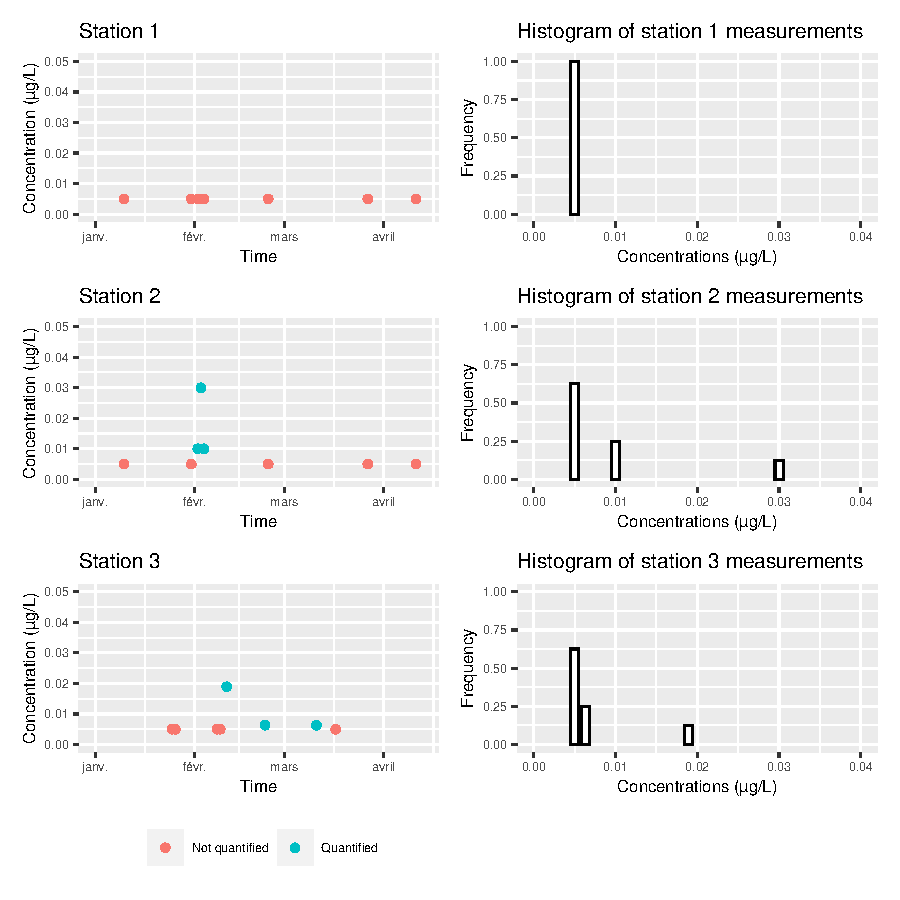
\includegraphics{figs/App/Simu_ex.pdf}
    \caption{Example of three stations data. The data were simulated.}
    \label{fig:ex_dist}
\end{figure}

The empirical 1-d Wasserstein distance used in our work is slightly adapted for left censored values. Given two samples $\bm{x}=(x_1,\dots,x_n)$ and $\bm{y}=(y_1,\dots,y_m)$ of sizes $n$ and $m$ with respective empirical c.d.f. $F_n$ and $G_m$, the 1-d empirical distance writes:
$$W_1(F_n,G_n) = \int_{\mathbbm{R}}\lvert F_n(x)-G_m(x) \rvert\mathrm{d}x$$
In the case of left censored observations, the empirical c.d.f. the first non zero value is the censoring threshold. If we use the classical empirical c.d.f., it does not take into account that the potential real values of censored samples is potentially lower than this threshold. In particular, if both samples $\bm{x}$ and $\bm{y}$ are fully censored at respective thresholds $a_1$ and $a_2$, the Wasserstein distance equals $\lvert a_1-a_2 \rvert$. We would like this quantity to be the smallest possible since none of the samples has any quantified values. Since the samples size for a single station is usually very small, a reasonable assumption is to suppose that the real values under the censoring threshold are uniformly distributed. Figure \ref{fig:mod_dist} illustrates the changes it implies on the empirical c.d.f.. In the previous example of $\bm{x}$ and $\bm{y}$, the adapted empirical distance gives $\lvert a_1-a_2\rvert/2$.    

\begin{figure}[H]
    \centering
    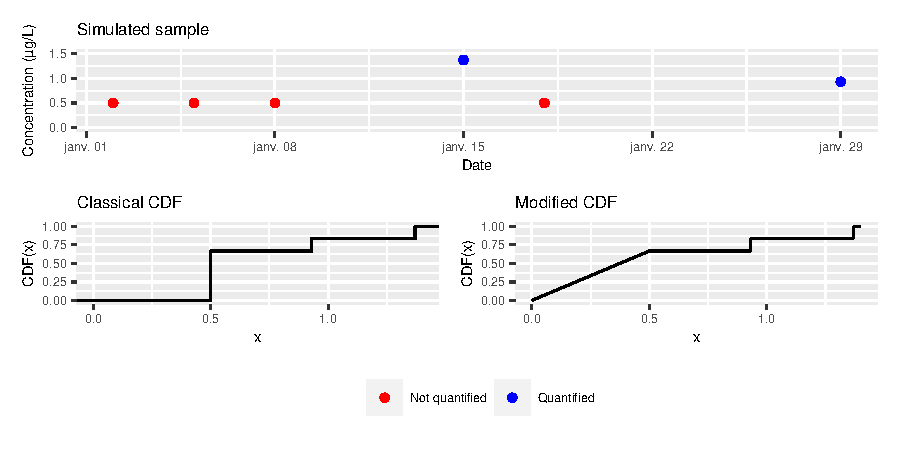
\includegraphics{figs/App/Wass_ew.pdf}
    \caption{Example of modified c.d.f. for the Wasserstein distance.}
    \label{fig:mod_dist}
\end{figure}

\section{Supplementary Figures}

\subsection{Regional map of crops}\label{section:crops}
The regional map of crops provided in Figure \ref{fig:crops} have been produced using data from the \emph{registre parcellaire graphique} produced by the IGN \cite{IGN:RPG}.

\begin{figure}[H]
    \centering
    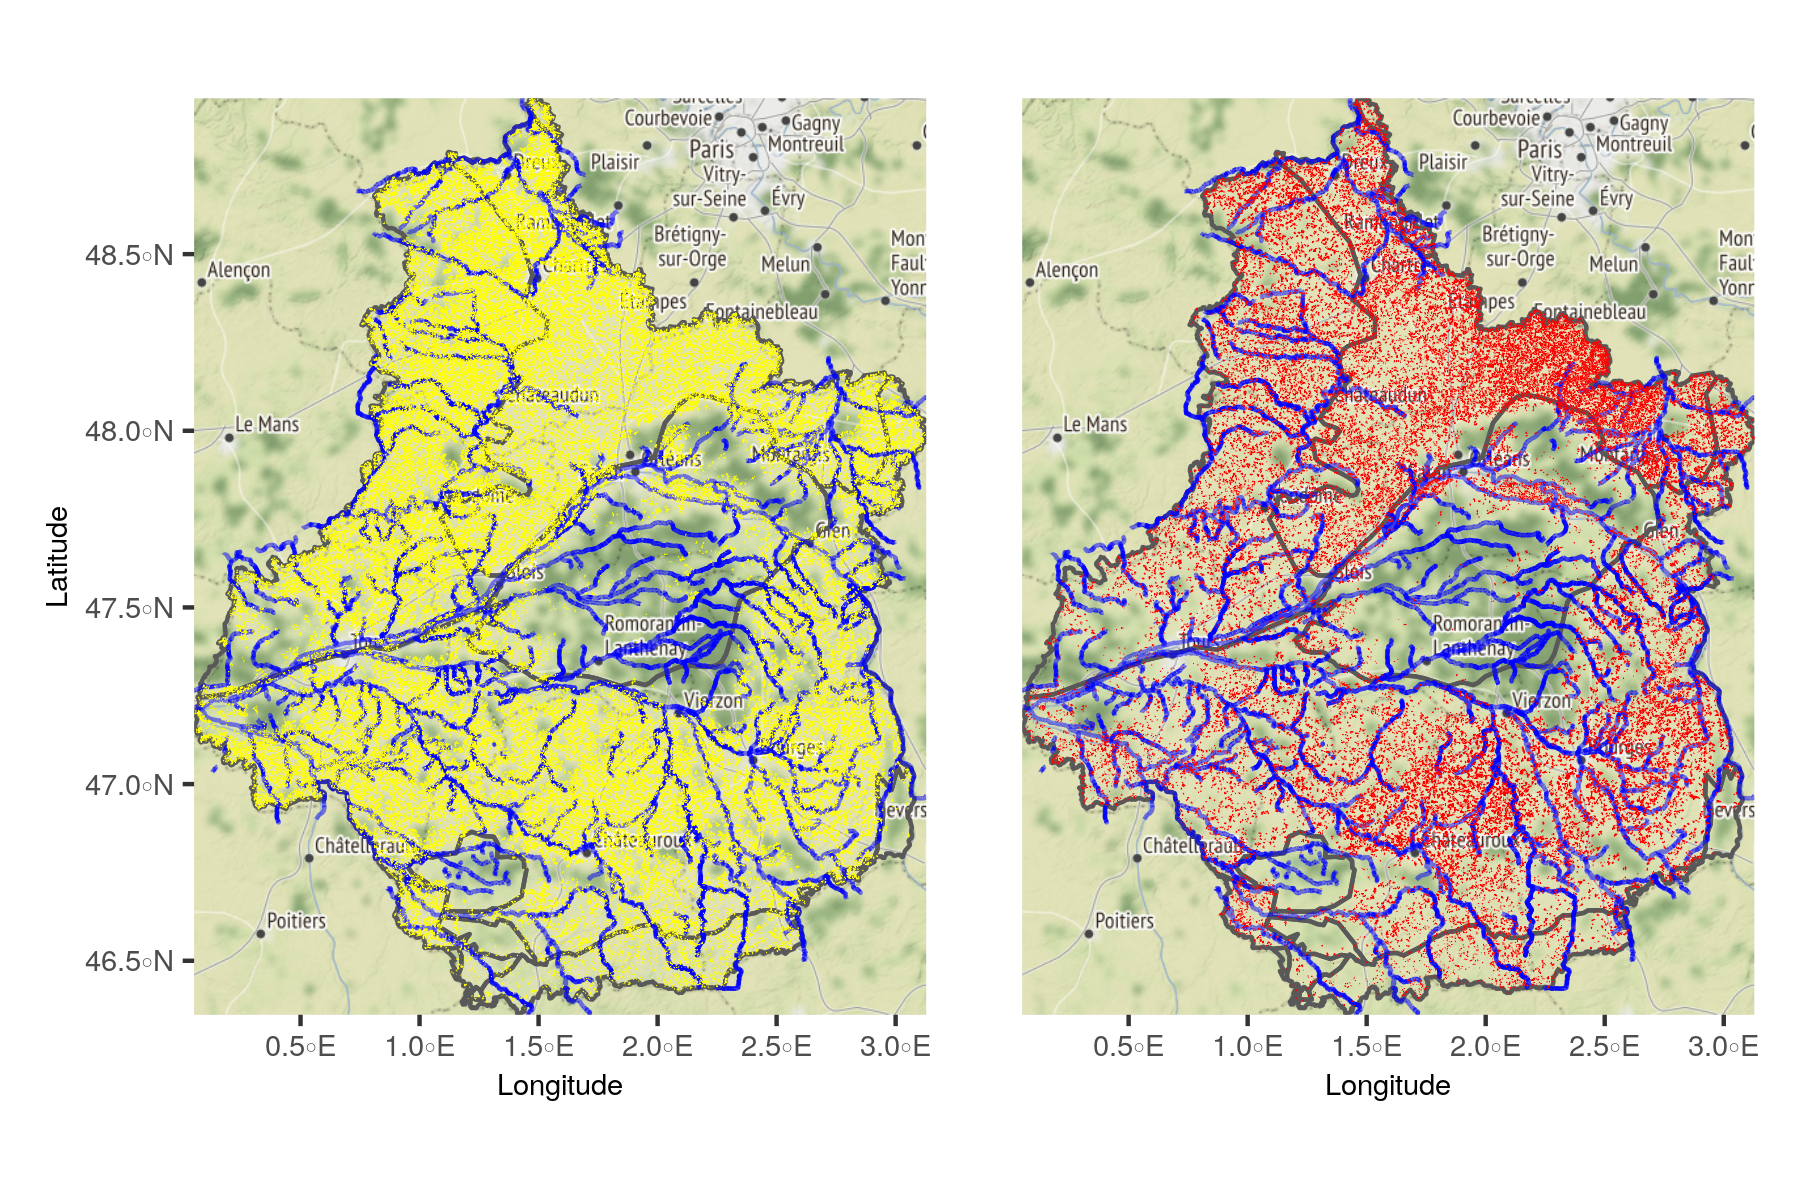
\includegraphics{figs/App/Occ_soil.png}
    \caption{Wheat (in yellow) and barley (in red) crops location in Centre-Val de Loire}
    \label{fig:crops}
\end{figure} 

\subsection{Prosulfocarb sales}\label{section:sale}

Prosulfocarb sales figures used to build Figure \ref{fig:sale} are made available by the \emph{Système d'information sur l'eau} \cite{BNVD}.

\begin{figure}[H]
  \centering
  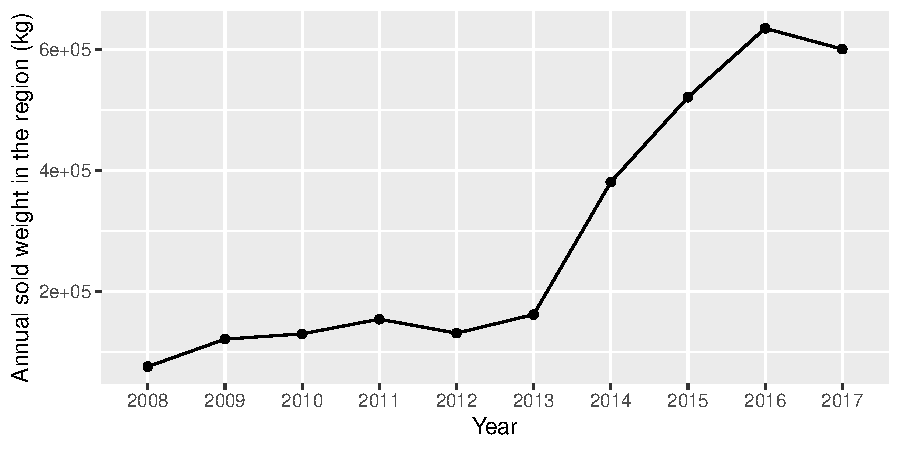
\includegraphics[]{figs/App/Sales_pro.pdf}
  \caption{Prosulfocarb sales between 2008 and 2017 in the Centre-Val de Loire region}
  \label{fig:sale}
\end{figure}

\subsection{All elbow methods figures}\label{section:elb}

\begin{figure}[H]
  \centering
  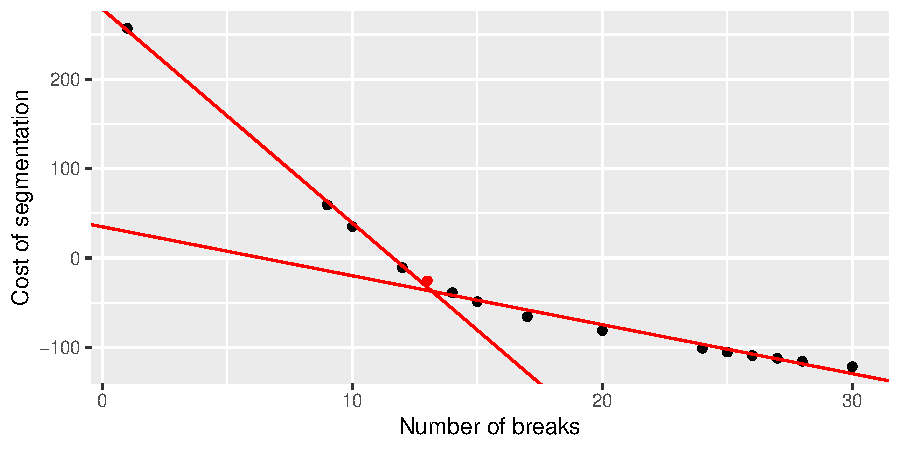
\includegraphics[]{figs/App/Elbow_seg.pdf}
  \caption{Elbow method selecting the optimal segmentation of the full signal $\overline{\mathcal{D}}$.}
  \label{fig:elb_seg}
\end{figure}

\begin{figure}[H]
  \centering
  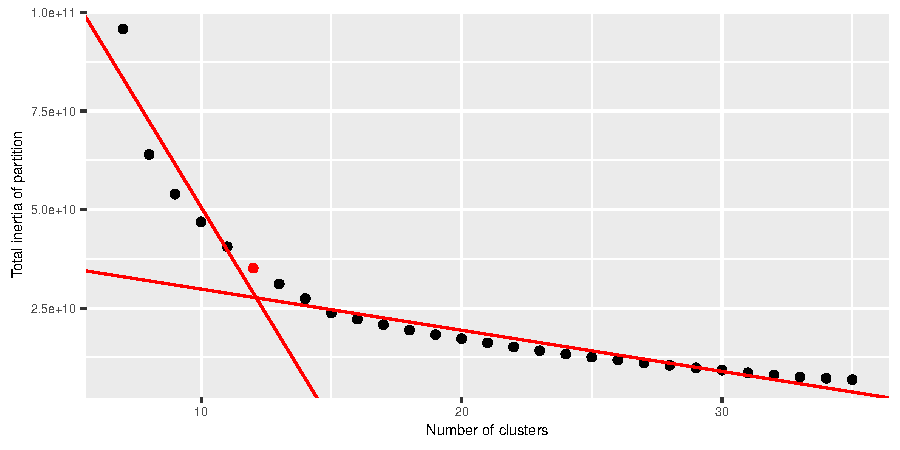
\includegraphics[]{figs/Chap5/Elb_clust.pdf}
  \caption{Elbow method for the spatial clustering.}
  \label{fig:elb:clust}
\end{figure}

\chapter{Chapter \ref{chp:6} supplementary material} \label{app:chap6}

\section{Clustering selected for the application}\label{app:chap6:1}

In order to choose the clusterings that are imported in to the application, we use the elbow method described in Algorithm \ref{chp:3:algoelbow}. Instead of plotting the clustering inertia values against their number of clusters, we use the logarithm of the inertia. The decrease of the inertia don't seem to have any linera behaviour. Two elbows appeared in the dicrease of the logratihm though.  

\begin{figure}[H]
  \centering
  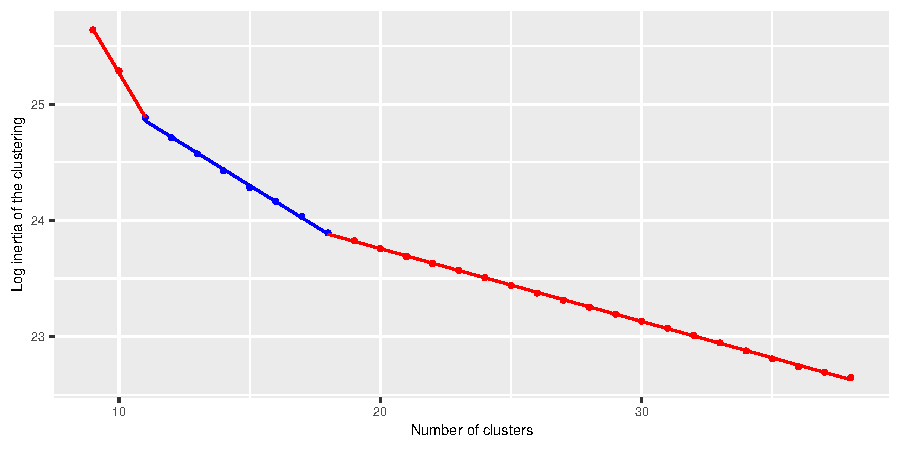
\includegraphics[]{figs/App/NB_CLUST.pdf}
  \caption{Clustering candidates selected in the application.}
  \label{fig:elb:clust}
\end{figure}

Instead of fitting a bipartite model, we fitted the best piece-wise linear model composed of three regression models as drawned in Figure \ref{fig:elb:clust}. All the clustering that had their log-inertia located on the middle regression line were selected. They are coloredin blue in Figure \ref{fig:elb:clust}.    

\section{Application explanatory note}\label{app:chap6:2}


\includepdf[pages=-, pagecommand={}]{8-Appendix/notice.pdf}

\end{appendices}